\documentclass[11pt]{article}
\usepackage[margin=1in]{geometry}
\usepackage{amsmath, amssymb}
\usepackage{graphicx}
\usepackage{float}
\usepackage{booktabs}
\usepackage[font=small,labelfont=bf]{caption}
\usepackage{subcaption}
\usepackage{xcolor}
\usepackage{hyperref}
\hypersetup{colorlinks=true,linkcolor=blue!60!black,urlcolor=blue!60!black}

\title{\Large\textbf{GAD vs Sella on HIP --- 3-method benchmark (reduced)}\\[4pt]
\normalsize 2026-04-28 reduced. Transition1x train, $n{=}300$, 6 noise levels,
2000 steps, $f_{\max}{<}0.01 \wedge n_{\text{neg}}{=}1$, IRC = \texttt{sella\_hip}.}
\author{}
\date{}

\begin{document}
\maketitle
\thispagestyle{empty}

\tableofcontents

% =================================================================
\newpage
\section{Headline}
% =================================================================

\begin{figure}[H]
\centering
\begin{subfigure}[t]{0.495\textwidth}
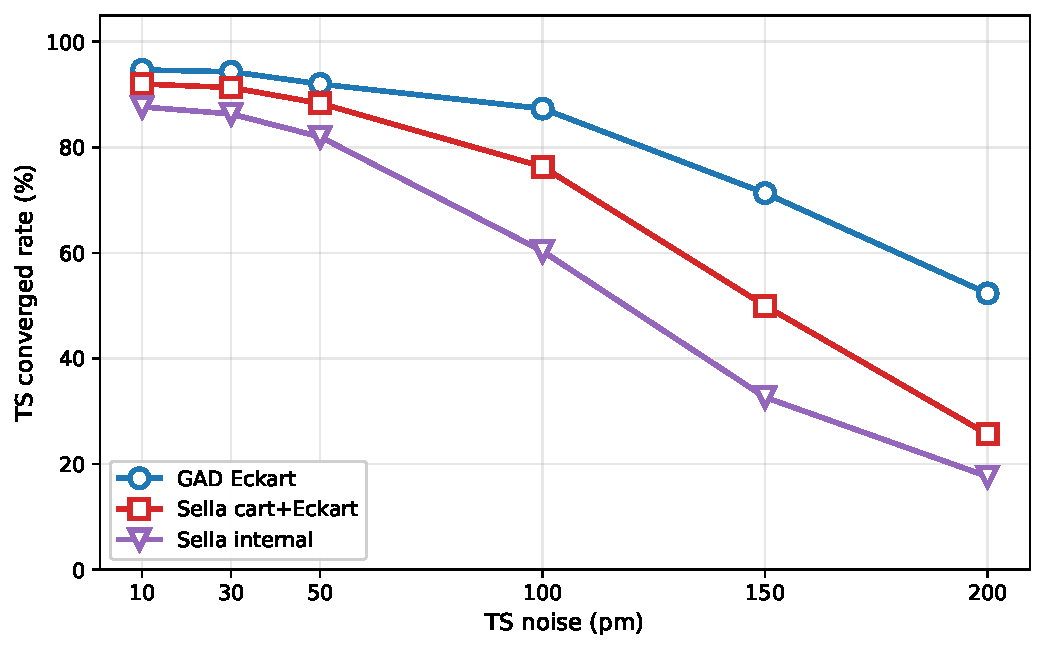
\includegraphics[width=\textwidth]{figures/fig_cmp_conv_3m.pdf}
\caption{TS-converged rate vs.\ noise.}
\end{subfigure}
\hfill
\begin{subfigure}[t]{0.495\textwidth}
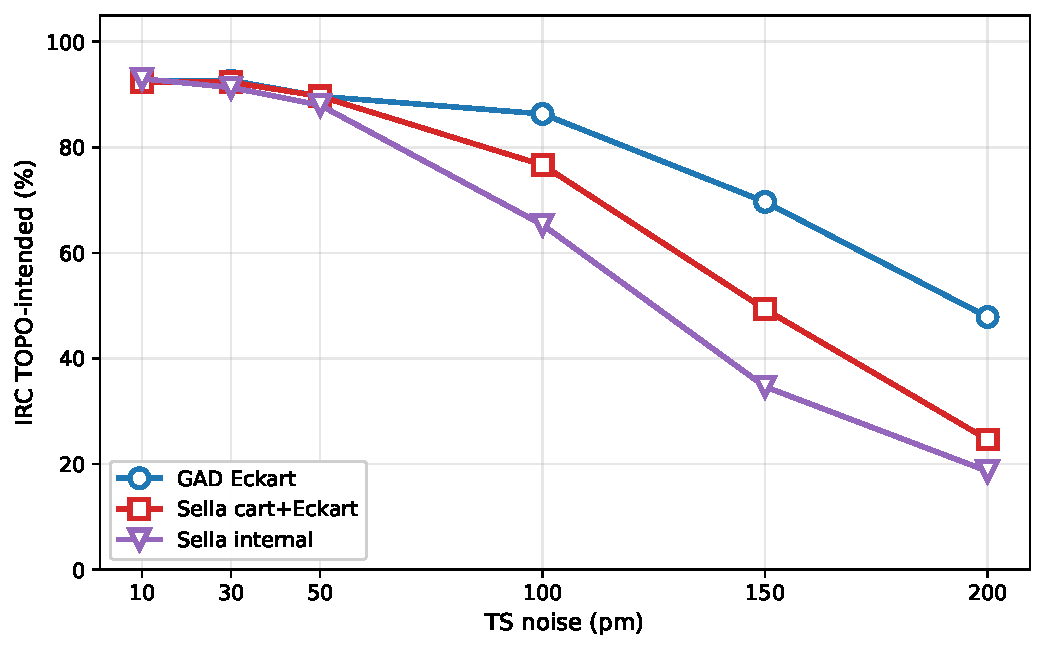
\includegraphics[width=\textwidth]{figures/fig_cmp_irc_topo_3m.pdf}
\caption{IRC TOPO-intended rate vs.\ noise.}
\end{subfigure}
\caption{Three canonical methods: GAD Eckart, Sella cart+Eckart, Sella internal.}
\end{figure}

\begin{figure}[H]
\centering
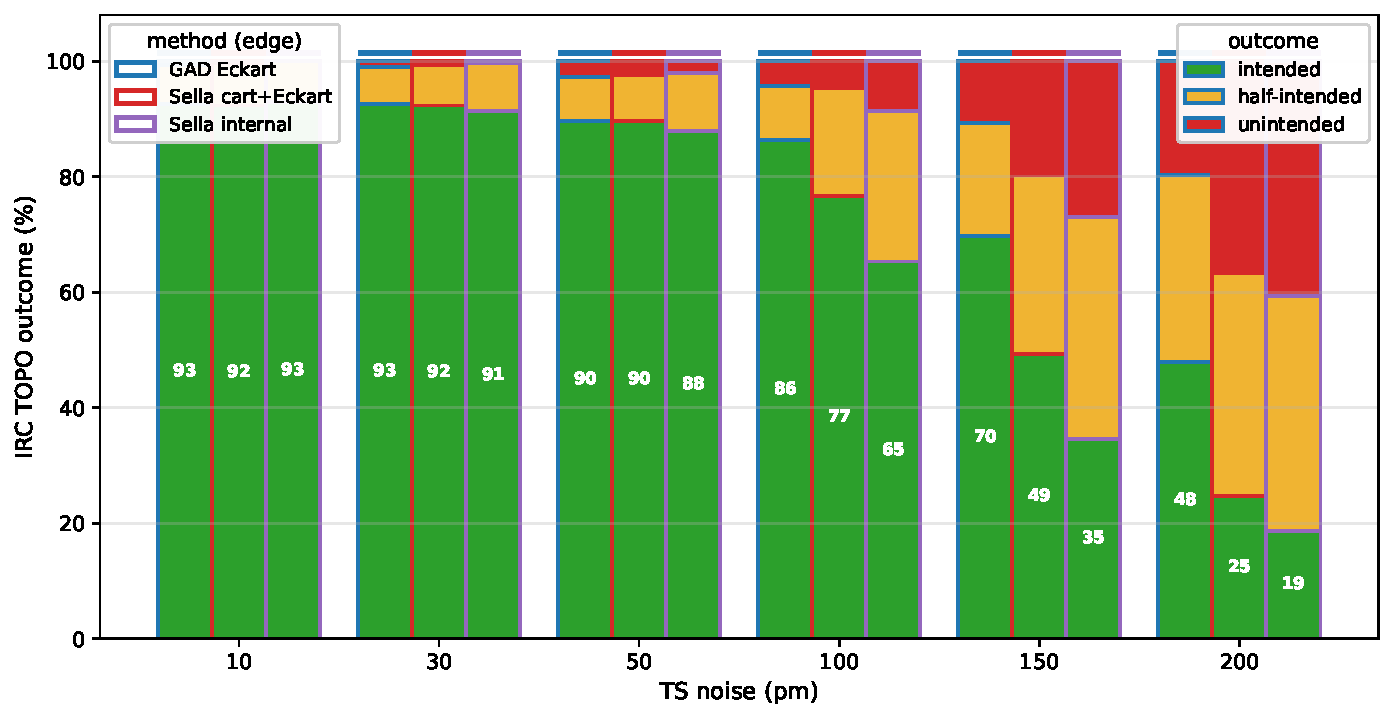
\includegraphics[width=\textwidth]{figures/fig_irc_intended_grouped_3m.pdf}
\caption{IRC TOPO outcome breakdown per method per noise.
Bar fill = outcome (intended / half / unintended). Bar edge color = method.}
\end{figure}

\begin{center}
\textbf{TS-converged rate (\%, $n{=}300$)}\\[0.3em]
\begin{tabular}{l|cccccc}
\toprule
Method & 10 & 30 & 50 & 100 & 150 & 200 \\
\midrule
GAD Eckart           & 87.3 & 87.3 & 85.3 & \textbf{80.0} & \textbf{63.7} & \textbf{45.3} \\
Sella cart$+$Eckart  & \textbf{92.0} & \textbf{91.3} & \textbf{88.3} & 76.3 & 50.0 & 25.7 \\
Sella internal       & 87.7 & 86.3 & 82.0 & 60.3 & 32.7 & 17.0 \\
\bottomrule
\end{tabular}
\vskip0.8em
\textbf{IRC TOPO-intended (\%, $n{=}300$)}\\[0.3em]
\begin{tabular}{l|cccccc}
\toprule
Method & 10 & 30 & 50 & 100 & 150 & 200 \\
\midrule
GAD Eckart           & \textbf{93.0} & \textbf{93.0} & \textbf{90.7} & \textbf{86.7} & \textbf{70.0} & \textbf{47.0} \\
Sella cart$+$Eckart  & 92.3 & 92.3 & 89.7 & 76.7 & 49.3 & 24.7 \\
Sella internal       & \textbf{93.0} & 91.3 & 88.0 & 65.3 & 34.7 & 18.7 \\
\bottomrule
\end{tabular}
\end{center}

\newpage
% =================================================================
\section{GAD step-size over time}
% =================================================================

\begin{figure}[H]
\centering
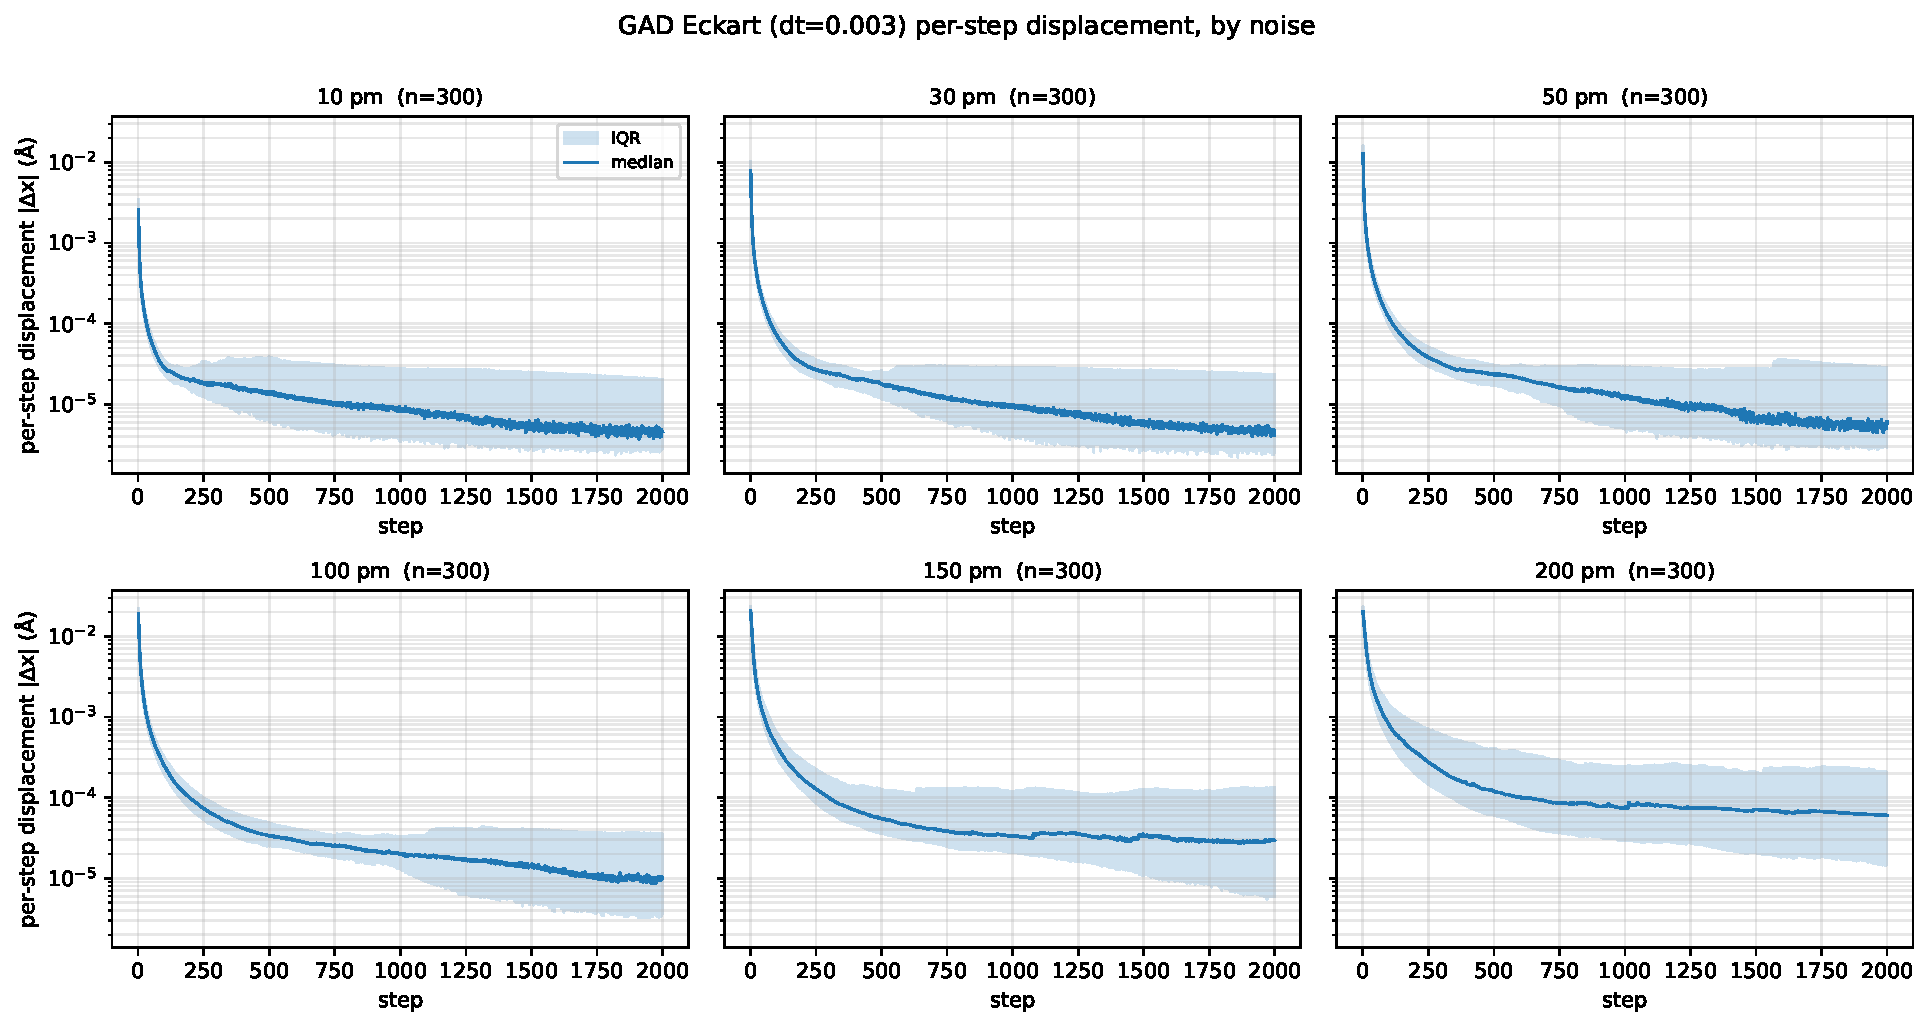
\includegraphics[width=\textwidth]{figures/fig_gad_stepsize_vs_step.pdf}
\caption{GAD Eckart (dt=0.003) per-step Cartesian displacement.
Median (line) and IQR (band), aggregated over 300 trajectories per noise.}
\end{figure}

\newpage
% =================================================================
\section{Per-method breakdown}
% =================================================================

\begin{figure}[H]
\centering
\begin{subfigure}[t]{0.495\textwidth}
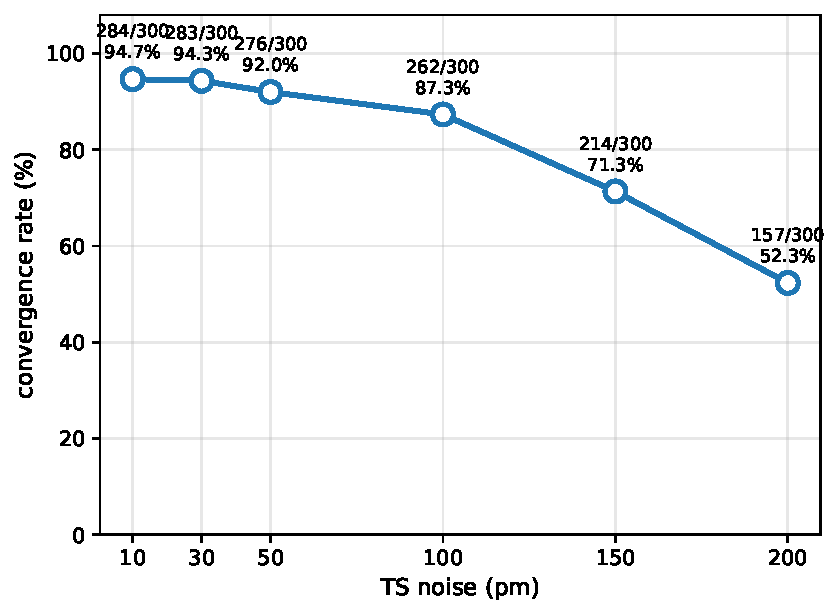
\includegraphics[width=\textwidth]{figures/fig_method_gad_eckart_conv_line.pdf}
\caption{GAD Eckart --- TS converged}
\end{subfigure}
\hfill
\begin{subfigure}[t]{0.495\textwidth}
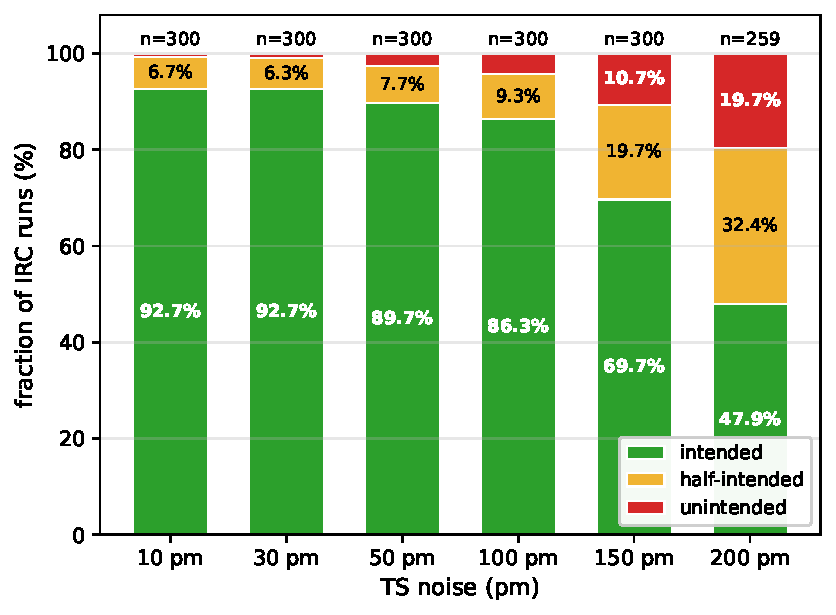
\includegraphics[width=\textwidth]{figures/fig_method_gad_eckart_irc_bars_topo.pdf}
\caption{GAD Eckart --- IRC TOPO}
\end{subfigure}
\caption{\texttt{gad\_dt003} with Eckart projection, $dt{=}0.003$, 2000 steps.}
\end{figure}

\begin{figure}[H]
\centering
\begin{subfigure}[t]{0.495\textwidth}
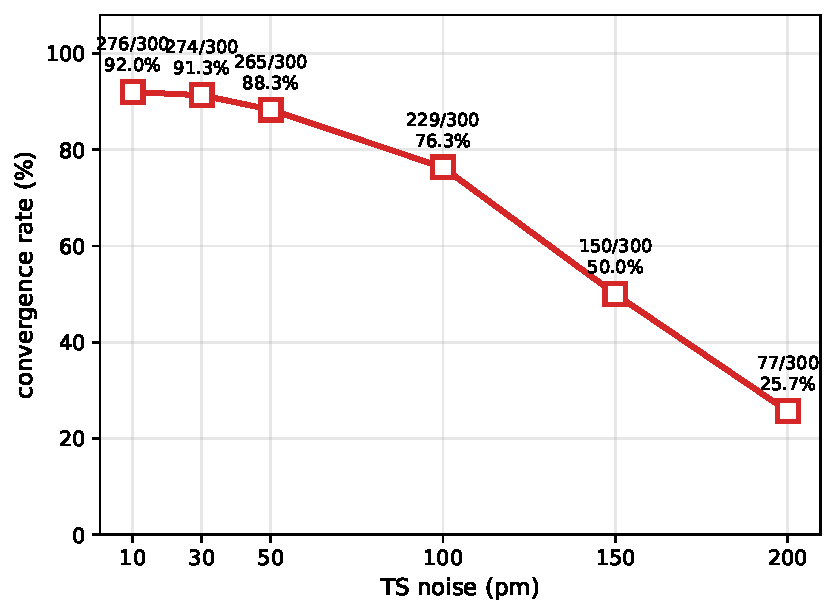
\includegraphics[width=\textwidth]{figures/fig_method_sella_carte_2k_conv_line.pdf}
\caption{Sella cart+Eckart --- TS converged}
\end{subfigure}
\hfill
\begin{subfigure}[t]{0.495\textwidth}
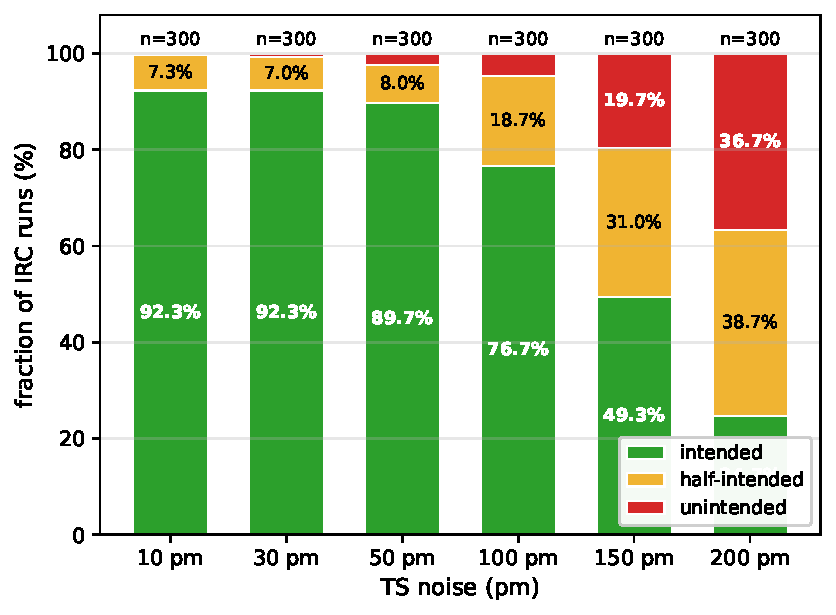
\includegraphics[width=\textwidth]{figures/fig_method_sella_carte_2k_irc_bars_topo.pdf}
\caption{Sella cart+Eckart --- IRC TOPO}
\end{subfigure}
\caption{Sella cartesian + Eckart, 2000 steps, HIP Hessian every step.}
\end{figure}

\begin{figure}[H]
\centering
\begin{subfigure}[t]{0.495\textwidth}
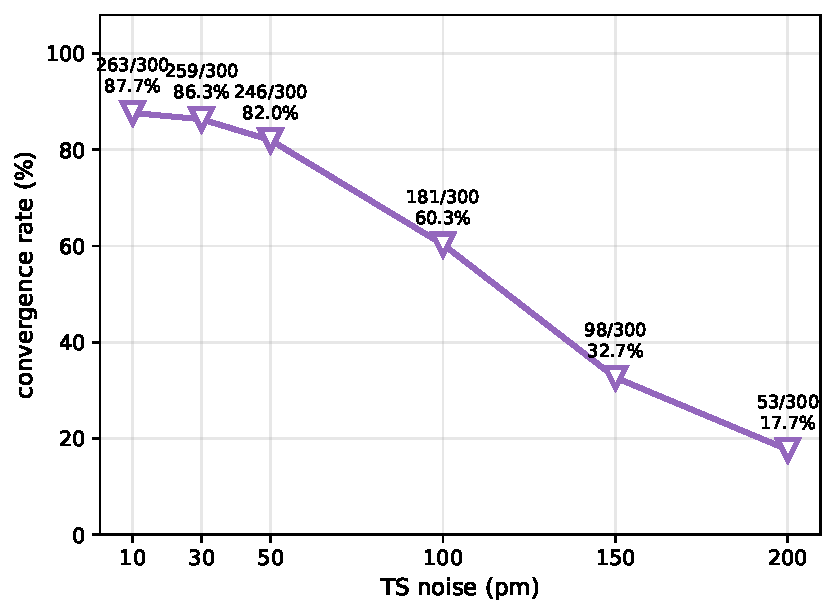
\includegraphics[width=\textwidth]{figures/fig_method_sella_int_2k_conv_line.pdf}
\caption{Sella internal --- TS converged}
\end{subfigure}
\hfill
\begin{subfigure}[t]{0.495\textwidth}
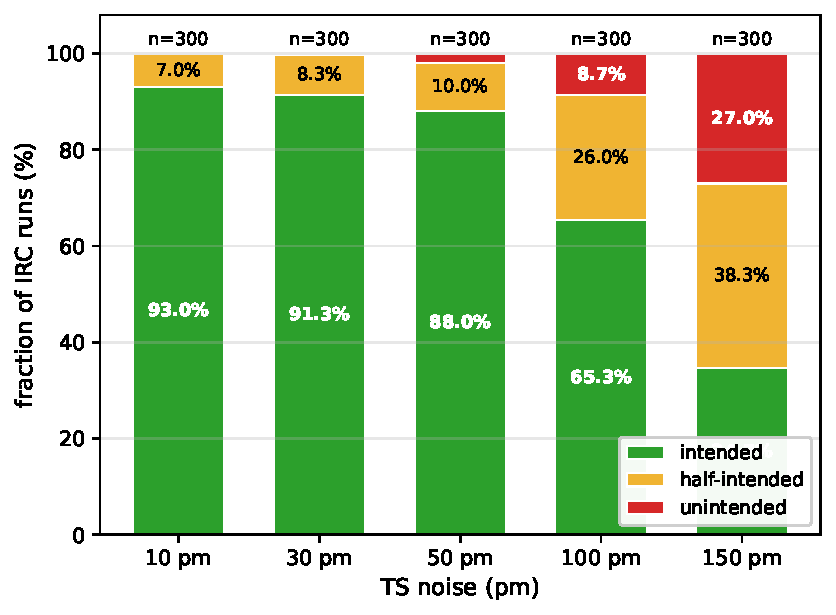
\includegraphics[width=\textwidth]{figures/fig_method_sella_int_2k_irc_bars_topo.pdf}
\caption{Sella internal --- IRC TOPO}
\end{subfigure}
\caption{Sella internal coords, 2000 steps, HIP Hessian every step.}
\end{figure}

\newpage
% =================================================================
\section{Criterion vs IRC sample overlap}
% =================================================================

\begin{figure}[H]
\centering
\begin{subfigure}[t]{0.48\textwidth}
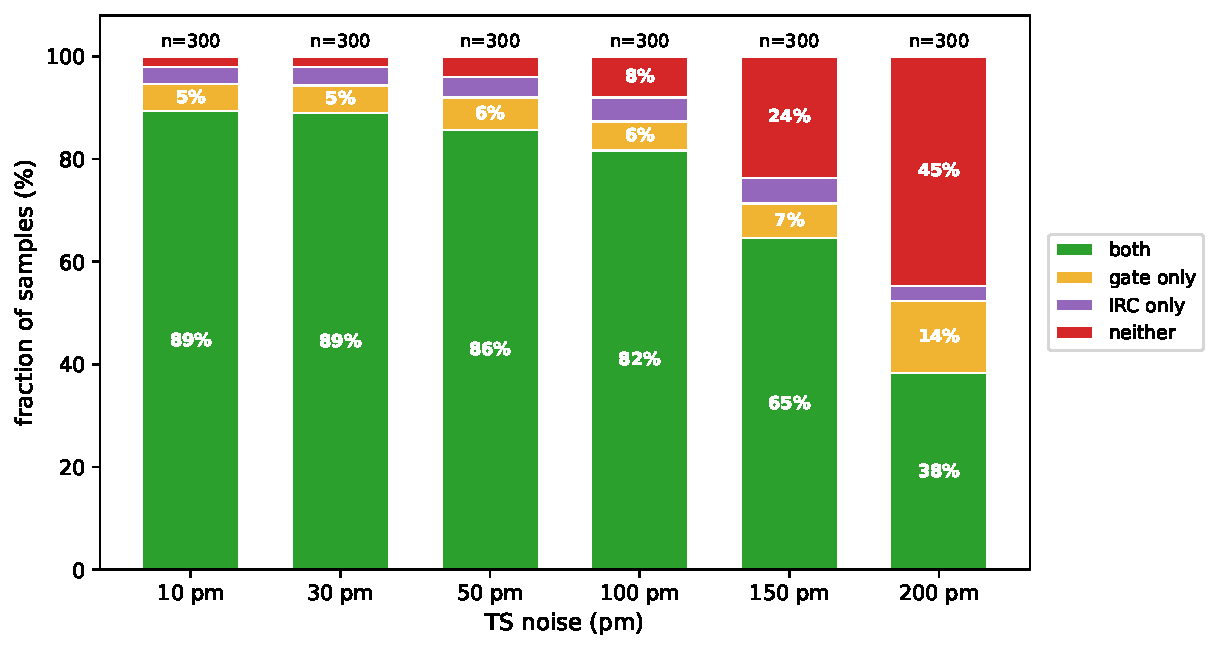
\includegraphics[width=\textwidth]{figures/fig_gate_vs_irc_gad_eckart.pdf}
\caption{GAD Eckart}
\end{subfigure}
\hfill
\begin{subfigure}[t]{0.48\textwidth}
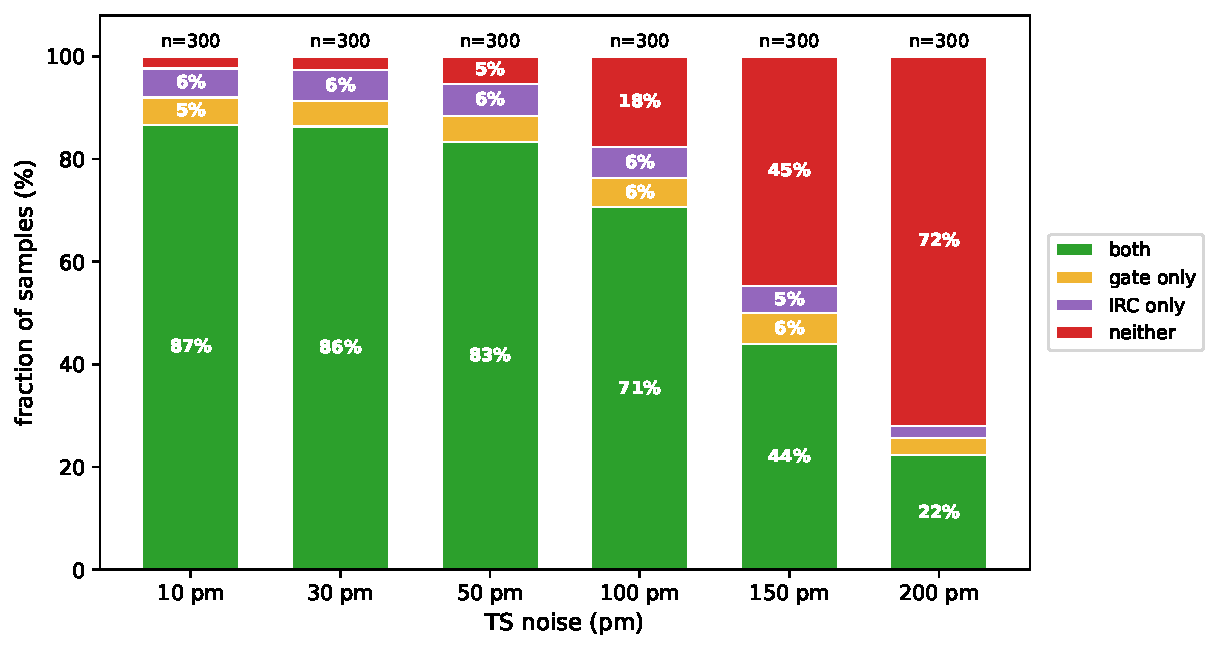
\includegraphics[width=\textwidth]{figures/fig_gate_vs_irc_sella_carte_2k.pdf}
\caption{Sella cart+Eckart}
\end{subfigure}
\vskip0.5em
\begin{subfigure}[t]{0.48\textwidth}
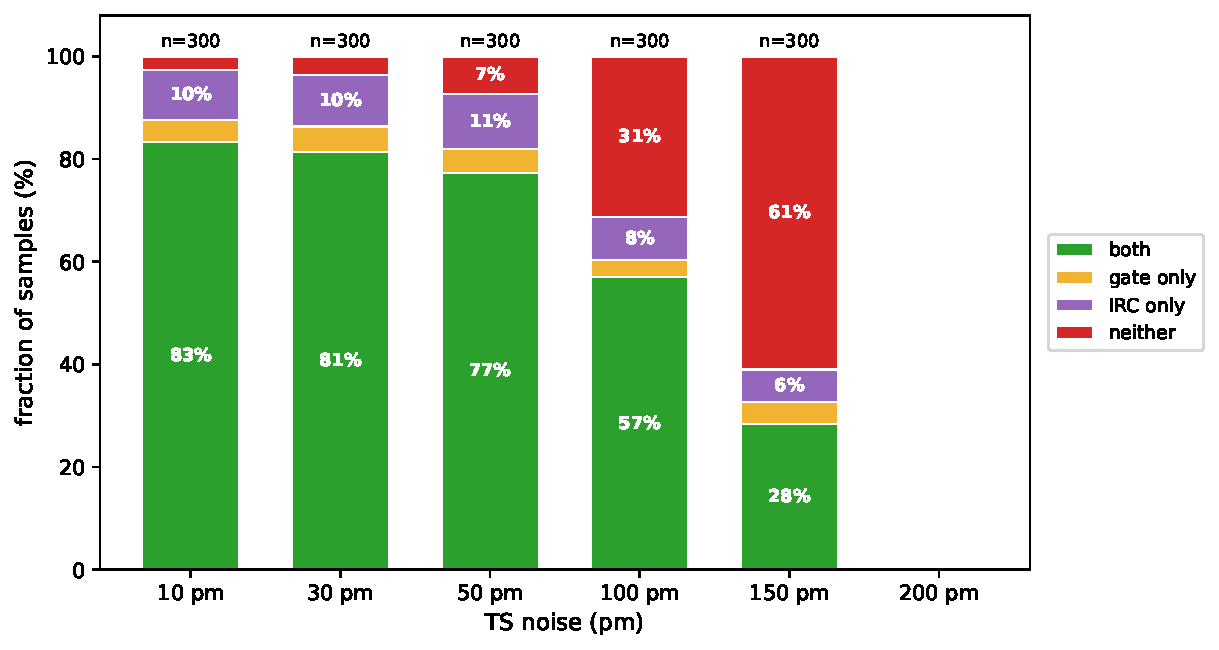
\includegraphics[width=\textwidth]{figures/fig_gate_vs_irc_sella_int_2k.pdf}
\caption{Sella internal}
\end{subfigure}
\caption{Per-method TS-converged vs.\ IRC-TOPO sample overlap.
Green = both pass. Yellow = converged only. Purple = IRC only. Red = neither.}
\end{figure}

\newpage
% =================================================================
\section{Data locations}
% =================================================================

\begin{center}
\begin{tabular}{ll}
\toprule
Artifact & Path \\
\midrule
GAD Eckart summaries           & \texttt{runs/round2/}, \texttt{round3/} \\
Sella cart+Eckart summaries    & \texttt{runs/sella\_2000/} \\
Sella internal summaries       & \texttt{runs/sella\_2000/} \\
GAD IRC                        & \texttt{runs/irc\_sellahip\_allendpoints/} \\
Sella cart+Eckart IRC          & \texttt{runs/irc\_sella\_carte\_2000/} \\
Sella internal IRC             & \texttt{runs/irc\_sella\_int\_2000/} \\
This report                    & \texttt{IRC\_COMPREHENSIVE\_2026-04-28-reduced.tex/pdf} \\
\bottomrule
\end{tabular}
\end{center}

\end{document}
